\chapter{Methods}

The study was divided in two parts, the first one corresponded to the
development of a simulation of an electromagnetic calorimeter in Geant4,
inspired in the design of ECAL in the LHCb experiment. With this simulation, a
data set was created. The events used high energetic electrons, photons and
neutral pions, as primary particles. This dataset was the input in the second
part of the study.

In the second part of the study, a machine learning implementation was used to
create a multivariable classifier that, using the measurements taken in the
simulation, categorize the events according to the primary particle.

\section{Simulation Description}

As explained previously, the electromagnetic calorimeter in the LHCb experiment
is divided in three sections, where the inner one detects signal from high
energetic particles. A detector inspired on the modules of the inner section
was simulated in Geant4. The calorimeter is composed by a mesh of \(6\times4\)
modules (see \cref{fig:cropped-geometry}). Each module is a combination of thin
layers of scintillator and lead. A total of 67 and 66 tiles for each material
correspondingly.

\begin{figure}[htb]
  \centering

  \subfloat[Detector simulation from the primary creation point.]{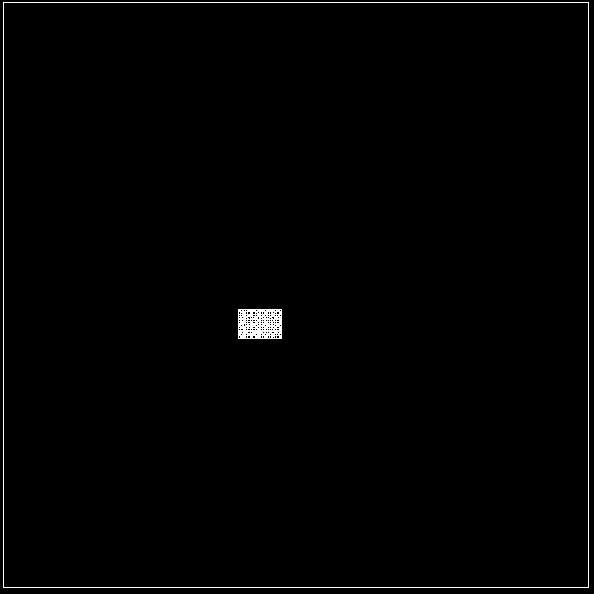
\includegraphics[scale=0.25]{Kap2/ecal-inner-section-cropped-geometry-1.png}\label{fig:cropped-geometry-1}}\hspace{2em}
  \subfloat[Detector simulation zoomed]{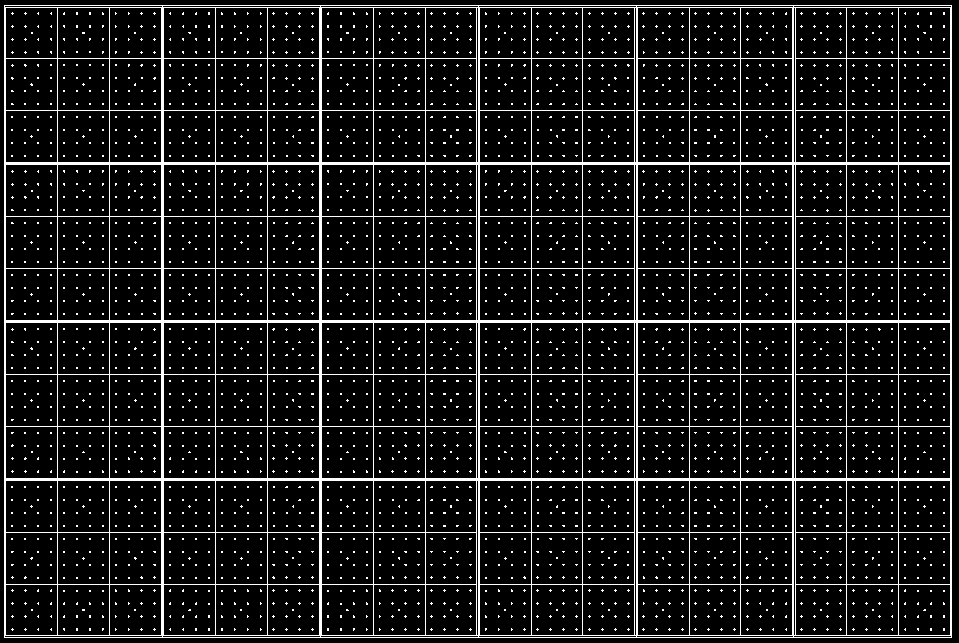
\includegraphics[scale=0.25]{Kap2/ecal-inner-section-cropped-geometry-2.png}\label{fig:cropped-geometry-2}}

  \caption{Front view of the detector. In \ref{fig:cropped-geometry-1}, the
  white square correspond to the caolrimeter and the black is the simulated
  void world box.}\label{fig:cropped-geometry}

\end{figure}

In each module, the scintillator tiles are divided in nine pieces of the same
size, making a mesh of \(3\times3\), while the lead tiles are whole pieces. All
of them have a set of holes as shown in the \cref{fig:module-geometry}, where
WSL wires are placed. All the modules have a recovery of stainless steel of
\(\SI{1}{\cm}\) thick.

\begin{figure}[htb]
  \centering

  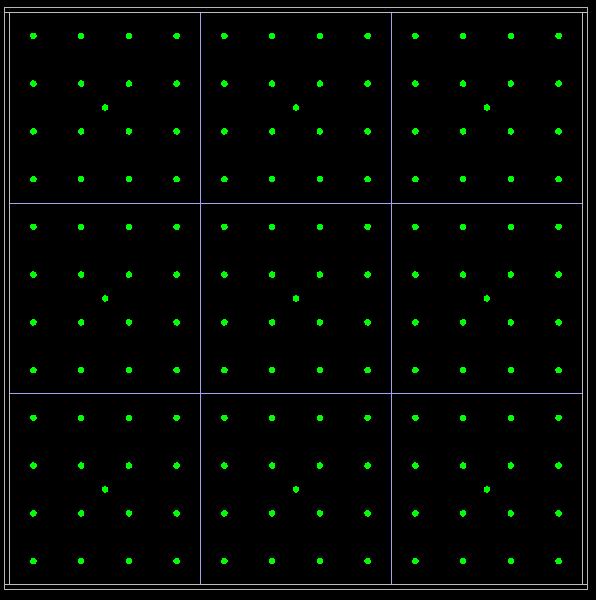
\includegraphics[scale=0.5]{Kap2/Mesh.png}
  \caption{Front view of a single detector module.}\label{fig:module-geometry}

\end{figure}

As explained above, electrons, photons and neutral pions of
\(\SI{20}{\giga\electronvolt}\) were used as primary particles. The primary
particle was placed \(\SI{13}{\metre}\) from the calorimeter.

For each event, the simulation collects information on the number of photons
and electrons created in each of the scintillator and lead layers. For this, it
stores the coordinates of the plate in the detector. It also saves the step
length and the energy deposited on each of the plates, for each interaction
between a particle and that layer. All this information is stored in a ROOT
file. A dataset with \(10000\) events per primary particle was created.

\section{Machine Learning Implementation}

\subsection{Kolmogorov Test}

It should be noted that not all calorimeter plates have photons or electrons
created in them, or in general no particles interact in these layers and
therefore do not contain any information, also the distribution of photons and
electrons created, the step length and the energy deposited in each of the
plates is the same for each of the primary particles, so it is not significant
when applying the classification algorithm. Because of this, a filter was
performed to obtain the significant cells, which will be taken into account in
the machine learning implementation.

A Kolmogorov test were applied for the distribution of all the measured
variables in each of the plates in the detector. This test is used to determine
whether the two histograms are compatible with the same
distribution\cite{root,kolmogorov}. Applying this test, the cells with similar
distributions will be excluded from the machine learning input, since they do
not add significant information to the classifier to separate the primary
particles. The cells that got less than \(0.5\) in the Kolmogorov test were
taken into account in the machine learning implementation.

\subsection{Machine Learning Algorithm}

The machine learning algorithm was built using the Scikit Learn library for
python. The following five multidimensional classifiers were used:
MultinomialNB, BernoulliNB, Perceptron, SGDClassifier,
PassiveAggressiveClassifier. MultinomialNB and BernoulliNB classifiers are both
Naive Bayes methods, that uses the Bayes’ theorem with the assumption that
every pair of features is independent of each other given the class
variable\cite{zhang2004optimality,NBsklearn,scikit-learn}. The difference
between the two algorithms is that the Bernoulli Naive Bayes method explicity
penalizes the non-occurrence of a feature that is an indicator of a given
class\cite{NBsklearn}.

The Perceptron and the PassiveAggressiveClassifier are Linear methods, it means
that they consider that the target class can be expressed as a lineal
combination of the features\cite{LMsklearn,scikit-learn}. Both methods do not
require a learning rate, but the the PassiveAggressiveClassifier includes a
regularizatión parameter while Perceptron does not. Finally, SGDClassifier use
the Stochastic Gradient Descent routing for fitting a linear classifier. It
allow the use of different loss functions and penalties for
classification\cite{SGDsklearn,scikit-learn}.

These classifiers were chosen due to the size of the input set, even after
getting information just from significant cells, the arrays were too large,
then it is computationally easier to partially fit the model with each new data
vector. The data from the simulation was divided in two groups, \(5000\) events
each one, that worked as train and test set respectively.
